%\documentstyle[epsf,twocolumn]{jarticle}       %LaTeX2e仕様
\documentclass[twocolumn]{jarticle}     %pLaTeX2e仕様(platex.exeの場合)
% \documentclass[onecolumn]{ujarticle}   %pLaTeX2e仕様(uplatex.exeの場合)
%%%%%%%%%%%%%%%%%%%%%%%%%%%%%%%%%%%%%%%%%%%%%%%%%%%%%%%%%%%%%%
%%
%%  基本バージョン
%%
%%%%%%%%%%%%%%%%%%%%%%%%%%%%%%%%%%%%%%%%%%%%%%%%%%%%%%%%%%%%%%%%
\setlength{\topmargin}{-45pt}
%\setlength{\oddsidemargin}{0cm}
\setlength{\oddsidemargin}{-7.5mm}
%\setlength{\evensidemargin}{0cm}
\setlength{\textheight}{24.1cm}
%setlength{\textheight}{25cm}
\setlength{\textwidth}{17.4cm}
%\setlength{\textwidth}{172mm}
\setlength{\columnsep}{11mm}

%\kanjiskip=.07zw plus.5pt minus.5pt


% 【節が変わるごとに (1.1)(1.2) … (2.1)(2.2) と数式番号をつけるとき】
%\makeatletter
%\renewcommand{\theequation}{%
%\thesection.\arabic{equation}} %\@addtoreset{equation}{section}
%\makeatother

%\renewcommand{\arraystretch}{0.95} 行間の設定
%%%%%%%%%%%%%%%%%%%%%%%%%%%%%%%%%%%%%%%%%%%%%%%%%%%%%%%%
%\usepackage{graphicx}   %pLaTeX2e仕様(\documentstyle ->\documentclass)
\usepackage[dvipdfmx]{graphicx}
\usepackage{subcaption}
\usepackage{multirow}
\usepackage{amsmath}
\usepackage{url}
\usepackage{ulem}
\usepackage{algorithm}
\usepackage{algorithmic}
\usepackage{listings} %,jlisting} %日本語のコメントアウトをする場合jlistingが必要
%ここからソースコードの表示に関する設定
\lstset{
  basicstyle={\ttfamily},
  identifierstyle={\small},
  commentstyle={\smallitshape},
  keywordstyle={\small\bfseries},
  ndkeywordstyle={\small},
  stringstyle={\small\ttfamily},
  frame={tb},
  breaklines=true,
  columns=[l]{fullflexible},
  numbers=left,
  xrightmargin=0zw,
  xleftmargin=3zw,
  numberstyle={\scriptsize},
  stepnumber=1,
  numbersep=1zw,
  lineskip=-0.5ex
}
%%%%%%%%%%%%%%%%%%%%%%%%%%%%%%%%%%%%%%%%%%%%%%%%%%%%%%%%
\begin{document}

	%bibtex用の設定
	%\bibliographystyle{ujarticle}

	\twocolumn[
		\noindent
		\hspace{1em}
		2020 年 8 月 28 日
		ゼミ資料
		\hfill
		B4 杉山 竜弥
		\vspace{2mm}

		\hrule
		\begin{center}
			{\Large \bf 進捗報告}
		\end{center}
		\hrule
		\vspace{9mm}
	]

	% ‚ここから 文章 Start!
\section{今週やったこと}
\begin{itemize}
	\item {コードの確認}
  \item {サーバで実験}
\end{itemize}

\section{コードの確認}
問題:演算子候補が偏って学習され, 精度が向上しない.

勾配の更新に不具合がある可能性を確かめるため, 本家とコードを比較.

コードを比較した結果, アーキテクチャの更新に種類があった.
1つは現在使っているコードと同じで通常のロス, もう1つは検証ロスで更新.
検証ロスの方が複雑なロジックで現在, コードを読みつつ, 実験中.

レイヤーの重みの訓練とアーキテクチャの訓練に使うデータを分離するのがカギかもしれない.

\subsection{論文のアーキテクチャで学習}
探索済みの設定で重みを学習して, どれくらいの精度ができかを確認.(図\ref{fig:nor}, \ref{fig:red})

\begin{figure}[tb]
	\begin{center}
		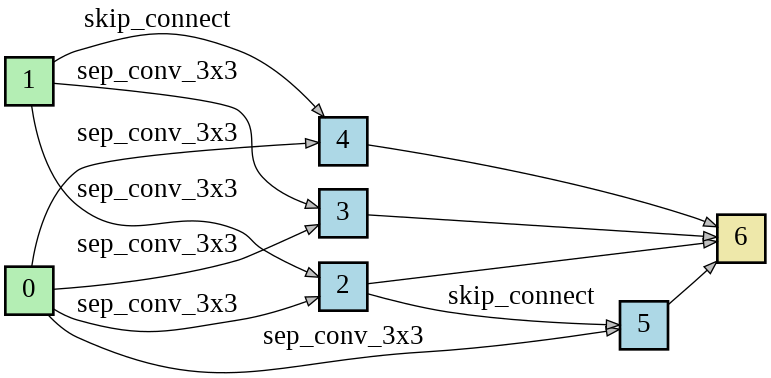
\includegraphics[clip,width=7.5cm]{complete_normal.png}
		\caption{探索済みのセル:normal}
		\label{fig:nor}
	\end{center}
\end{figure}
\begin{figure}[tb]
	\begin{center}
		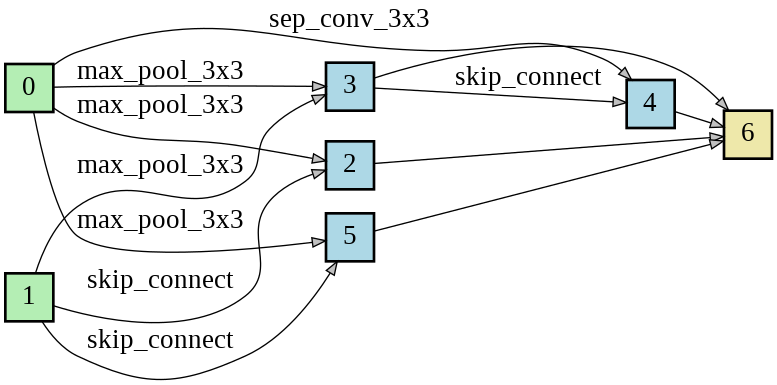
\includegraphics[clip,width=7.5cm]{complete_reduce.png}
		\caption{探索済みのセル:reduce}
		\label{fig:red}
	\end{center}
\end{figure}

結果:精度 75.8\%

% さすがに低すぎるので, 設定を見直す.
本家には遠く及ばない結果となった. 探索以外の細かい設定の違いがありそうなので, バグの存在とともに確認する.

\begin{table}[tb]
  \begin{center}
    \caption{実験の設定}
    \begin{tabular}{|c|c|} \hline
      Cell & 6 \\ \hline
      Node & 7(input=2, output=1) \\ \hline
      Optim(model) & SGD(lr=2.5e-2, momentum=0.9) \\ \hline
      Optim($\theta$) & Adam(lr=2e-4, $\beta$=(0.5, 0.999)) \\ \hline
      Loss & Cross Entropy Loss \\ \hline
      batch size & 64 \\ \hline
      train data & 20000 \\ \hline
      epoch & 50 \\ \hline
    \end{tabular}
    \label{tab:setting}
  \end{center}
\end{table}

% \section{考察}

\section{今後の予定}
% なんとなくなんかの勉強をするとかではなく具体的に
\begin{itemize}
  \item コードの確認
\end{itemize}

\section{ソースコード}
% 埋め込みでもGitでもいいので参照できるように
Githubの同階層の\url{NAS_test.ipynb}を参照してください.

% 参考文献リスト
\bibliographystyle{unsrt}
\bibliography{ref}
\end{document}
